\documentclass{article}[10 pt]
\usepackage{graphicx} % Required for inserting images
\usepackage{tikz}

\usetikzlibrary {arrows.meta,bending,positioning}
\title{Arrow bending}



\begin{document}
\maketitle

\section*{Example}

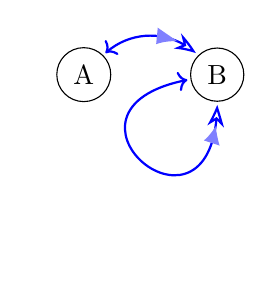
\begin{tikzpicture}
  \node [circle,draw] (A)              {A};
  \node [circle,draw] (B) [right=of A] {B};

  \draw [draw = blue, thick,
         arrows={
           Computer Modern Rightarrow [sep]
         - Latex[blue!50,length=8pt,bend,line width=0pt]
           Stealth[length=8pt,open,bend,sep]}]
    (A) edge [bend left=45] (B)
    (B) edge [in=-90, out=-170,looseness=12] (B);

\end{tikzpicture}


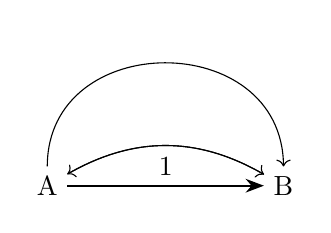
\begin{tikzpicture}
    % Nodes
    \node (A) at (0,0) {A};
    \node (B) at (3,0) {B};

    % Straight Arrow
    \draw[->,>={Stealth[]}, thick] (A) to node[above]{1} (B);
  
    % Bending Arrows
    \draw[->, bend left] (A) to (B);
    \draw[->, bend right] (B) to (A);
    
    % Custom Bending Arrow
    \draw[->] (A) .. controls +(up:2cm) and +(up:2cm) .. (B);
\end{tikzpicture}\\ \\


%copilot = wrong
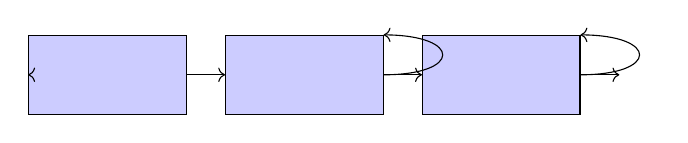
\begin{tikzpicture}
    % Draw the rectangles
    \node[draw, fill=blue!20, minimum width=2cm, minimum height=1cm] (A) at (0,0) {};
    \node[draw, fill=blue!20, minimum width=2cm, minimum height=1cm] (B) at (2.5,0) {};
    \node[draw, fill=blue!20, minimum width=2cm, minimum height=1cm] (C) at (5,0) {};
    
    % Draw the arrows
    \draw[->,] (-1,0) -- (A);
    \draw[->] (A) -- (B);
    \draw[->] (B) -- (C);
    \draw[->] (C) -- (6.5,0);
    
    % Draw the feedback loops
    \draw[->] (C.east) .. controls +(right:1cm) and +(right:1cm) .. (C.east |- A.north);
    \draw[->] (B.east) .. controls +(right:1cm) and +(right:1cm) .. (B.east |- A.north);
\end{tikzpicture}\\ \\


%miskat
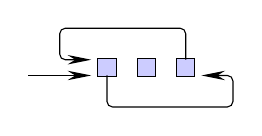
\begin{tikzpicture}[fill=blue!20]
  \node[rectangle,draw,fill] (a) at (0,0) {};
  \node[rectangle,draw,fill] (b) at (0.5,0) {};
  \node[rectangle,draw,fill] (c) at (1,0) {};
  
  \draw[-{Stealth[length=0.3cm,width=0.12cm]},rounded corners=2pt]       (0,-0.1) |- (1.6,-0.5) |- (1.2,-0.1); % down arrow
  
  \draw[-{Stealth[length=0.3cm,width=0.12cm]},rounded corners=2pt] (1,0.1)|-(-0.6,0.5)--(-0.6,0.1)--(-0.2,0.1);% up arrow
  \draw[-{Stealth[length=0.3cm,width=0.12cm]},rounded corners=2pt] (-1,-0.1)--(-0.2,-0.1);
\end{tikzpicture}\\ 



% My code
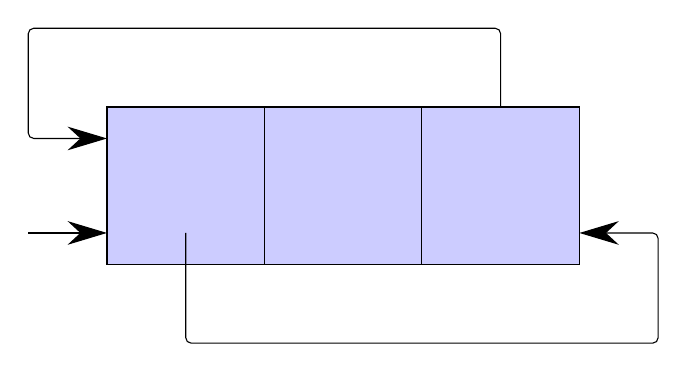
\begin{tikzpicture}
    \node[rectangle,draw,fill=blue!20, minimum width=2 cm, minimum height=2 cm] (a) at (0,0) {};
    \node[rectangle,draw,fill=blue!20, minimum width=2 cm, minimum height=2 cm] (b) at (2,0) {};
    \node[rectangle,draw,fill=blue!20, minimum width=2 cm, minimum height=2 cm] (c) at (4,0) {};

    \draw[-{Stealth[length=0.5cm, width=0.3cm]}, rounded corners = 2 pt] (0,-0.6) |- (6,-2) |- (5,-0.6);
    \draw[-{Stealth[length=0.5cm, width=0.3cm]}, rounded corners = 2 pt] (4,1) |- (-2,2) |- (-1,0.6);
    \draw[-{Stealth[length=0.5cm, width=0.3cm]}, rounded corners = 2 pt] (-2,-0.6) -- (-1,-0.6);
\end{tikzpicture}\\
\end{document}
